\documentclass[11pt,a4paper]{article}

% ===== Kodowanie i język =====
\usepackage[T1]{fontenc}
\usepackage[utf8]{inputenc}
\usepackage[polish]{babel}
\usepackage{lmodern}

% ===== Układ strony =====
\usepackage[a4paper,margin=2.5cm]{geometry}

% ===== Matematyka =====
\usepackage{amsmath, amssymb, amsfonts, amsthm, mathtools}

% ===== Grafika i rysunki =====
\usepackage{graphicx}
\usepackage{float}
\usepackage{xcolor}
\usepackage{tikz}

% ===== Algorytmy =====
\usepackage{algorithm}
\usepackage{algpseudocode}

% ===== Listy =====
\usepackage{enumitem}

% ===== Linki =====
\usepackage{hyperref}

% ===== Listing kodu =====
\usepackage{listings}

\lstset{
    basicstyle=\ttfamily\small,
    breaklines=true,
    frame=single,
    numbers=left,
    numberstyle=\tiny,
    stepnumber=1,
    numbersep=8pt,
    showstringspaces=false,
    tabsize=4
}

% ===== Skróty matematyczne =====
\newcommand{\R}{\mathbb{R}}
\newcommand{\Z}{\mathbb{Z}}
\newcommand{\N}{\mathbb{N}}
\newcommand{\Q}{\mathbb{Q}}
\newcommand{\C}{\mathbb{C}}
\newcommand{\D}{\mathcal{D}}
\newcommand{\F}{\mathbb{F}}

% ===== Środowiska twierdzeń =====
\theoremstyle{plain}
\newtheorem{tw}{Twierdzenie}[section]
\newtheorem{lem}[tw]{Lemat}
\newtheorem{wn}[tw]{Wniosek}

\theoremstyle{definition}
\newtheorem{df}[tw]{Definicja}
\newtheorem{uw}[tw]{Uwaga}
\newtheorem{prz}[tw]{Przykład}

% ===== Ustawienia linków =====
\hypersetup{
    colorlinks=true,
    linkcolor=blue,
    citecolor=blue,
    urlcolor=blue
}

\title{Lista 6: Chaos w sensie Devaneya\\Sprawozdanie (zadania 1--8)}
\author{Układy dynamiczne 8}
\date{\today}

\begin{document}

\maketitle
\tableofcontents

\section{Wstęp}

Sprawozdanie obejmuje zadania 1--8 z listy dotyczącej chaosu w sensie Devaneya.
W kolejnych punktach analizujemy między innymi przesunięcie Bernoulliego,
odwzorowanie namiotowe, odwzorowanie logistyczne oraz przekształcenie Gaussa,
sprawdzając własności dynamiki i podając przykłady klasycznych układów chaotycznych.

\section{Zadanie 1}

Niech
\[
x = (1,0,1,1,0,0,\dots).
\]
Wówczas kolejne iteracje przesunięcia są równe
\[
\sigma(x) = (0,1,1,0,0,\dots),
\]
\[
\sigma^2(x) = (1,1,0,0,\dots),
\]
\[
\sigma^3(x) = (1,0,0,\dots).
\]
Z definicji operatora $\sigma$ usuwa on pierwszy wyraz ciągu i przesuwa pozostałe o jedno miejsce w lewo, więc po trzech iteracjach otrzymujemy dokładnie powyższe ciągi.

Teraz sprawdzamy, czy ciąg
\[
y = (1,0,1,0,1,0,\dots)
\]
jest punktem okresowym. Mamy
\[
\sigma(y) = (0,1,0,1,0,\dots),
\]
\[
\sigma^2(y) = (1,0,1,0,1,0,\dots) = y.
\]
Zatem $y$ jest punktem okresowym dla $\sigma$ o okresie równym $2$. Nie jest to punkt stały, ponieważ $\sigma(y) \neq y$.

\section{Zadanie 2}

Niech
\[
T(x) = 1 - 2\left|x - \frac{1}{2}\right|.
\]
Wartości w podanych punktach obliczamy bezpośrednio:
\[
T(0) = 1 - 2\left|0 - \frac{1}{2}\right| = 0,
\]
\[
T\left(\frac{1}{4}\right) = 1 - 2\left|\frac{1}{4} - \frac{1}{2}\right| = \frac{1}{2},
\]
\[
T\left(\frac{1}{2}\right) = 1 - 2\left|\frac{1}{2} - \frac{1}{2}\right| = 1,
\]
\[
T\left(\frac{3}{4}\right) = 1 - 2\left|\frac{3}{4} - \frac{1}{2}\right| = \frac{1}{2},
\]
\[
T(1) = 1 - 2\left|1 - \frac{1}{2}\right| = 0.
\]

Równoważnie można zapisać
\[
T(x) =
\begin{cases}
2x, & x \in \left[0, \frac{1}{2}\right], \\
2 - 2x, & x \in \left[\frac{1}{2}, 1\right].
\end{cases}
\]
Z tego opisu od razu widać, że lewa połówka przedziału $[0,1]$ jest odwzorowywana na $[0,1]$ oraz prawa połówka także na $[0,1]$. Stąd
\[
T\left(\left[0, \frac{1}{2}\right]\right) = [0,1],
\qquad
T\left(\left[\frac{1}{2}, 1\right]\right) = [0,1].
\]

\begin{figure}[H]
    \centering
    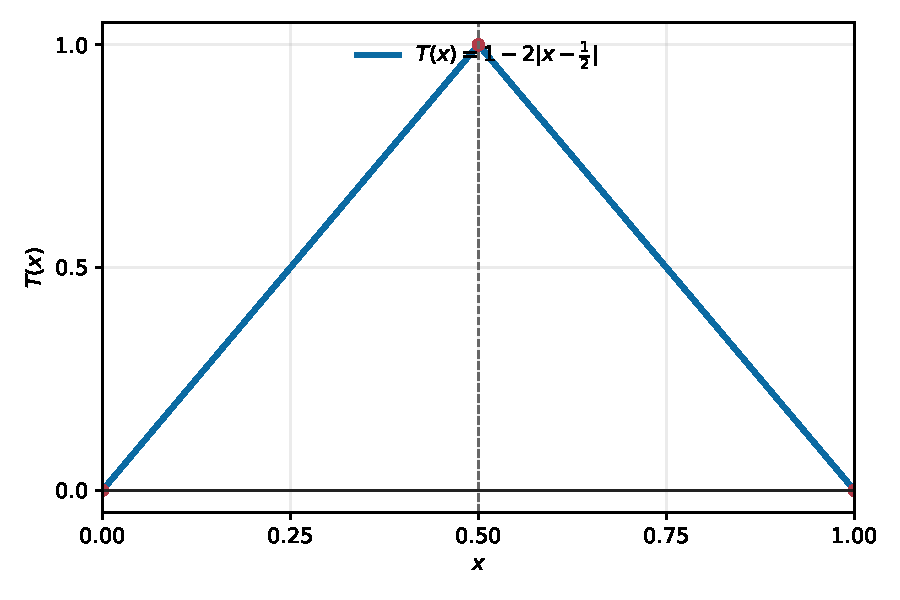
\includegraphics[width=0.78\linewidth]{figures/tent_map.pdf}
    \caption{Szkic odwzorowania namiotowego $T(x) = 1 - 2\left|x - \frac{1}{2}\right|$ na przedziale $[0,1]$.}
\end{figure}

\section{Zadanie 3}

Niech
\[
f(x) = 4x(1-x).
\]
Wtedy
\[
f(0) = 0,
\qquad
f\left(\frac{1}{4}\right) = 4\cdot \frac{1}{4}\cdot \frac{3}{4} = \frac{3}{4},
\]
\[
f\left(\frac{1}{2}\right) = 4\cdot \frac{1}{2}\cdot \frac{1}{2} = 1,
\qquad
f\left(\frac{3}{4}\right) = 4\cdot \frac{3}{4}\cdot \frac{1}{4} = \frac{3}{4},
\]
\[
f(1) = 0.
\]

Wygodnie jest też zapisać
\[
f(x) = 1 - 4\left(x - \frac{1}{2}\right)^2,
\]
więc wykres na $[0,1]$ jest parabolą o wierzchołku w punkcie $\left(\frac{1}{2}, 1\right)$.

\begin{figure}[H]
    \centering
    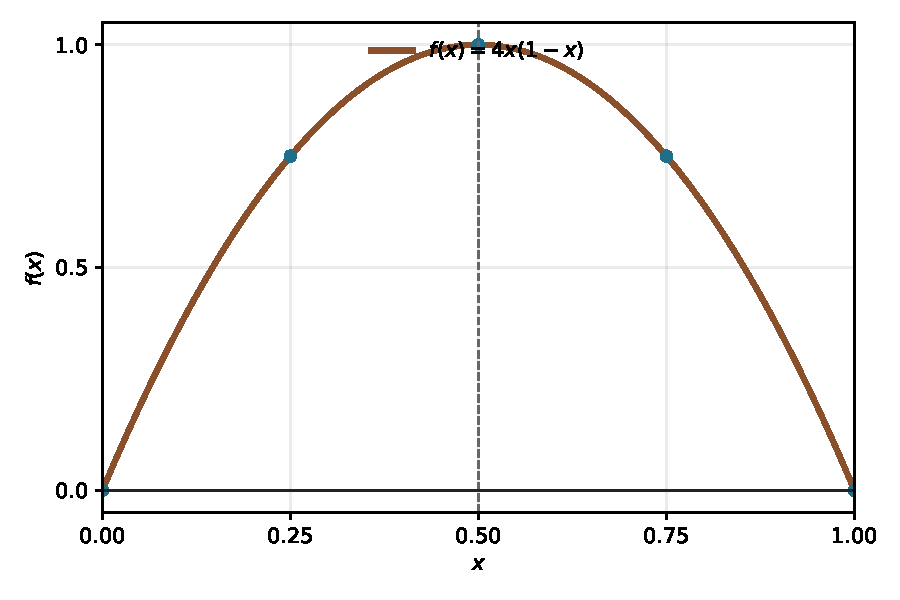
\includegraphics[width=0.78\linewidth]{figures/logistic_map.pdf}
    \caption{Szkic odwzorowania logistycznego $f(x)=4x(1-x)$ na przedziale $[0,1]$.}
\end{figure}

Sprawdźmy teraz tożsamość
\[
f(\sin^2\theta) = \sin^2(2\theta).
\]
Podstawiamy $x = \sin^2\theta$ i dostajemy
\[
f(\sin^2\theta) = 4\sin^2\theta\, (1-\sin^2\theta) = 4\sin^2\theta\cos^2\theta.
\]
Korzystając ze wzoru $\sin(2\theta)=2\sin\theta\cos\theta$, mamy
\[
4\sin^2\theta\cos^2\theta = \bigl(2\sin\theta\cos\theta\bigr)^2 = \sin^2(2\theta),
\]
co kończy sprawdzenie.

Korzystając z tej zależności, wygenerowano także wykresy iteracji $f^{(n)}$ dla kilku wartości $n$.

\begin{figure}[H]
    \centering
    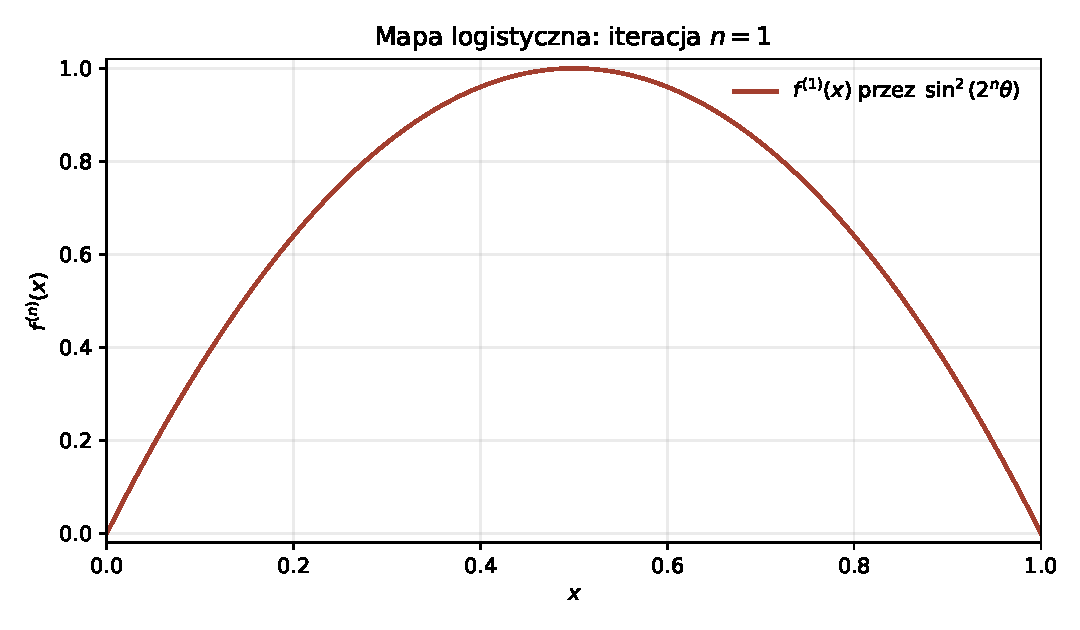
\includegraphics[width=0.82\linewidth]{figures/logistic_iterate_n1.pdf}
    \caption{Wykres iteracji $f^{(1)}$ mapy logistycznej wyznaczony wzorem trygonometrycznym.}
\end{figure}

\begin{figure}[H]
    \centering
    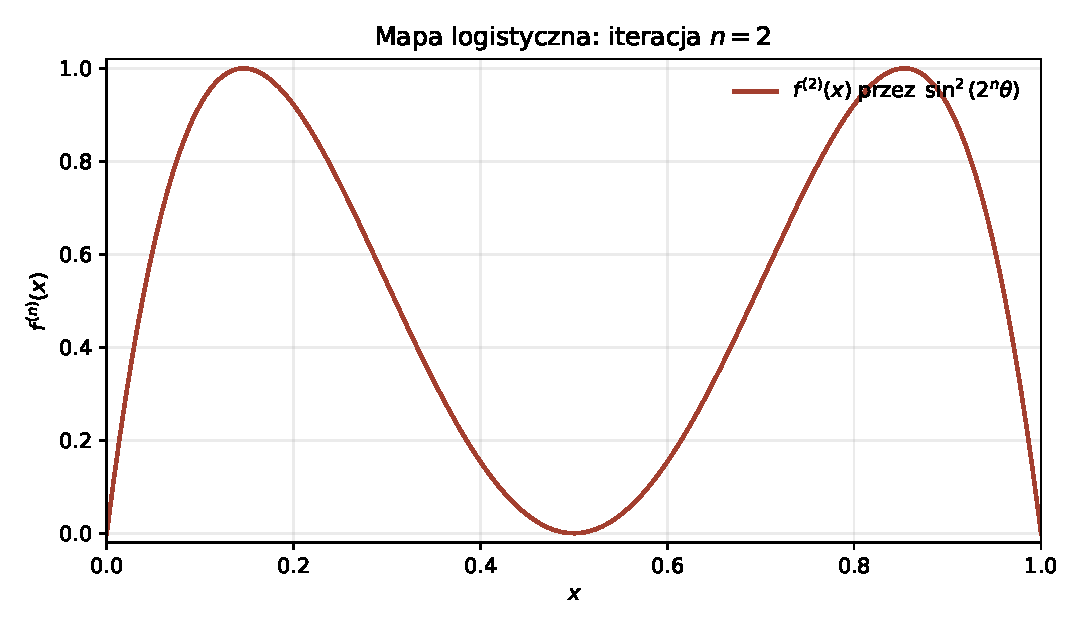
\includegraphics[width=0.82\linewidth]{figures/logistic_iterate_n2.pdf}
    \caption{Wykres iteracji $f^{(2)}$ mapy logistycznej wyznaczony wzorem trygonometrycznym.}
\end{figure}

\begin{figure}[H]
    \centering
    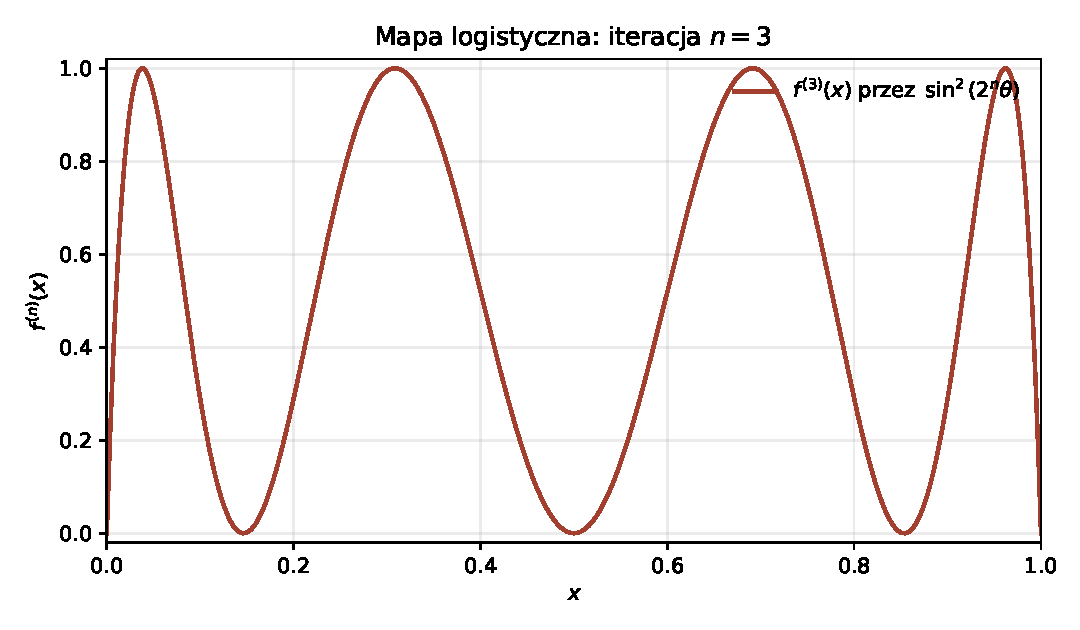
\includegraphics[width=0.82\linewidth]{figures/logistic_iterate_n3.pdf}
    \caption{Wykres iteracji $f^{(3)}$ mapy logistycznej wyznaczony wzorem trygonometrycznym.}
\end{figure}

\begin{figure}[H]
    \centering
    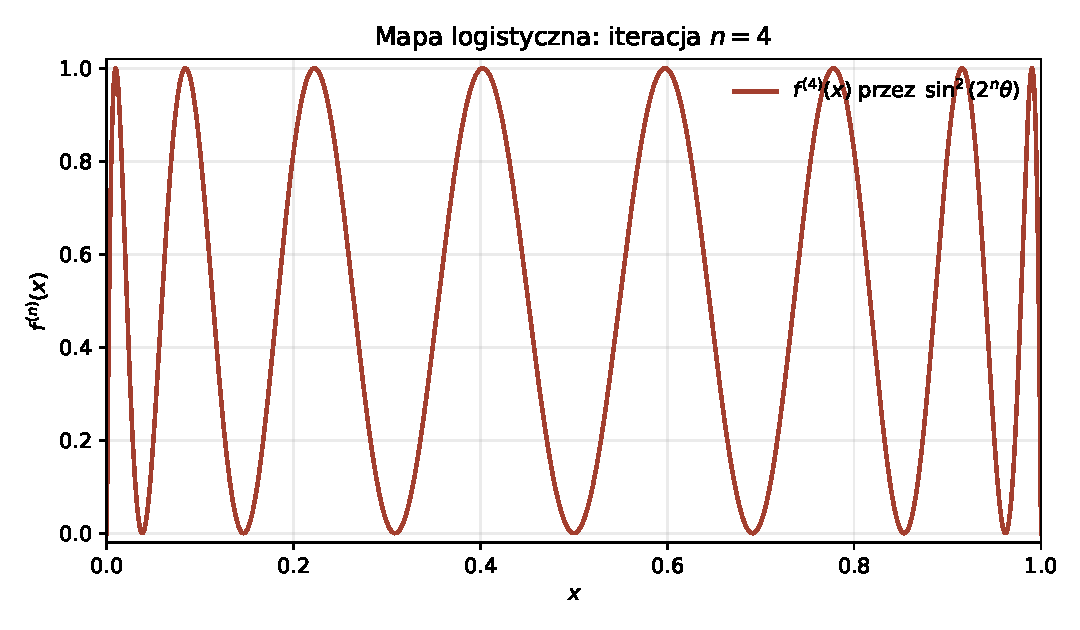
\includegraphics[width=0.82\linewidth]{figures/logistic_iterate_n4.pdf}
    \caption{Wykres iteracji $f^{(4)}$ mapy logistycznej wyznaczony wzorem trygonometrycznym.}
\end{figure}

\subsection*{Kod wykorzystany do generacji wykresów iteracji}

\lstinputlisting[language=Python,caption={Skrypt \texttt{logistic\_iterate\_trig.py} użyty do generacji wykresów $f^{(n)}$.}]{scripts/logistic_iterate_trig.py}

\section{Zadanie 4}

Rozważamy przestrzeń
\[
X = \{0,1\}^{\mathbb{Z}_{\ge 0}},
\qquad
d(x,y)=\sum_{i=0}^{\infty}\frac{|x_i-y_i|}{2^{i+1}},
\]
oraz przesunięcie Bernoulliego
\[
\sigma(x_0,x_1,x_2,\dots)=(x_1,x_2,x_3,\dots).
\]

Najpierw zauważmy, że $\sigma$ jest ciągłe (wprost: $d(\sigma x,\sigma y)\le 2d(x,y)$).
Pokażemy trzy własności Devaneya.

\textbf{1. Topologiczna tranzytywność (nawet mieszanie).}

Niech $U,V\subset X$ będą niepuste zbiory otwarte. W tej przestrzeni wystarczy rozpatrywać cylindry:
\[
U=[u_0\dots u_{p-1}],\qquad V=[v_0\dots v_{q-1}].
\]
Wybierzmy $n\ge p$ i zbudujmy punkt
\[
z=(u_0,\dots,u_{p-1},\underbrace{0,\dots,0}_{n-p\text{ razy}},v_0,\dots,v_{q-1},\dots).
\]
Wtedy $z\in U$, a po $n$ przesunięciach początek ciągu to $(v_0,\dots,v_{q-1})$, więc
\[
\sigma^n(z)\in V.
\]
Zatem $\sigma^n(U)\cap V\neq\varnothing$.

\textbf{2. Gęstość punktów okresowych.}

Weźmy dowolny cylinder $C=[a_0\dots a_{m-1}]$. Ciąg okresowy
\[
\bar a=(a_0,\dots,a_{m-1},a_0,\dots,a_{m-1},\dots)
\]
ma okres dzielący $m$ i należy do $C$. Każdy niepusty zbiór otwarty zawiera cylinder, a więc zawiera punkt okresowy. Punkty okresowe są więc gęste w $X$.

\textbf{3. Wrażliwość na warunki początkowe.}

Pokażemy ją bezpośrednio z definicji. Ustalmy $\delta=\tfrac12$. Niech $x\in X$ i $\varepsilon>0$. Wybierzmy $m$ tak, aby $2^{-(m+1)}<\varepsilon$, i zdefiniujmy $y\in X$ przez:
\[
y_i=x_i\ \text{dla } i\neq m,
\qquad
y_m=1-x_m.
\]
Wtedy
\[
d(x,y)=\frac{1}{2^{m+1}}<\varepsilon.
\]
Po $m$ iteracjach różnica trafia na pierwszy wyraz:
\[
\sigma^m(x)_0=x_m\neq y_m=\sigma^m(y)_0,
\]
więc
\[
d(\sigma^m(x),\sigma^m(y))\ge \frac12=\delta.
\]
To dokładnie wrażliwość na warunki początkowe.

Spełnione są więc wszystkie warunki chaosu Devaneya, zatem $\sigma$ jest chaotyczne w sensie Devaneya na $(X,d)$.

\section{Zadanie 5}

Rozważamy
\[
T:[0,1]\to[0,1],
\qquad
T(x)=1-2\left|x-\frac12\right|.
\]
Jest to odwzorowanie ciągłe i odcinkowo liniowe o dwóch gałęziach:
\[
T(x)=2x \text{ na } \left[0,\frac12\right],
\qquad
T(x)=2-2x \text{ na } \left[\frac12,1\right].
\]

Wygodnie wprowadzić gałęzie odwrotne
\[
g_0(y)=\frac y2,\qquad g_1(y)=1-\frac y2,
\]
czyli $T\circ g_i=\mathrm{id}_{[0,1]}$.

Dla słowa $w=(w_0,\dots,w_{n-1})\in\{0,1\}^n$ definiujemy
\[
I_w := g_{w_0}\circ g_{w_1}\circ\cdots\circ g_{w_{n-1}}([0,1]).
\]
Wtedy $I_w$ jest przedziałem długości $2^{-n}$, a $T^n$ odwzorowuje $I_w$ na całe $[0,1]$.

\textbf{1. Tranzytywność topologiczna (nawet dokładność topologiczna).}

Niech $U\subset[0,1]$ będzie niepusty i otwarty. Wybieramy $n$ tak duże, aby $2^{-n}<|U|$. Ponieważ przedziały $I_w$ (dla $|w|=n$) tworzą podział $[0,1]$ na drobne kawałki, istnieje słowo $w$ takie, że $I_w\subset U$.
Stąd
\[
T^n(U)\supset T^n(I_w)=[0,1].
\]
W szczególności dla dowolnego niepustego otwartego $V$ mamy $T^n(U)\cap V\neq\varnothing$.

\textbf{2. Gęstość punktów okresowych.}

Niech $U$ będzie niepustym przedziałem otwartym. Jak wyżej bierzemy $I_w\subset U$ dla pewnego słowa $w$ długości $n$.
Rozważmy słowa powtarzane periodycznie: $w^k$ i odpowiadające przedziały zagnieżdżone
\[
I_w\supset I_{w^2}\supset I_{w^3}\supset\cdots.
\]
Ich długości dążą do zera, więc przekrój zawiera dokładnie jeden punkt $x\in I_w\subset U$.
Z konstrukcji trajektoria $x$ ma periodyczny kod o okresie $n$, zatem $T^n(x)=x$.
Każde niepuste otwarte $U$ zawiera więc punkt okresowy.

\textbf{3. Wrażliwość na warunki początkowe.}

Z punktów 1 i 2 mamy, że $T$ jest tranzytywne i ma gęsty zbiór punktów okresowych. Przestrzeń $[0,1]$ jest nieskończoną przestrzenią metryczną, więc z twierdzenia Banksa wynika wrażliwość na warunki początkowe.

Spełnione są wszystkie warunki Devaneya, zatem $T$ jest chaotyczne w sensie Devaneya na $[0,1]$.

\section{Zadanie 6}

Rozważamy odwzorowanie logistyczne
\[
f:[0,1]\to[0,1],
\qquad
f(x)=4x(1-x).
\]
Z zadania 5 wiemy już, że odwzorowanie namiotowe
\[
T(x)=1-2\left|x-\frac12\right|
\]
jest chaotyczne w sensie Devaneya. Pokażemy, że $f$ jest z nim sprzężone topologicznie.

Definiujemy
\[
h:[0,1]\to[0,1],
\qquad
h(x)=\sin^2\!\left(\frac{\pi x}{2}\right).
\]
Funkcja $h$ jest homeomorfizmem (ciągła, ściśle rosnąca, z ciągłą odwrotnością na $[0,1]$).

Sprawdzamy relację sprzężenia:
\[
f\circ h = h\circ T.
\]
Rzeczywiście,
\[
f(h(x))
=4\sin^2\!\left(\frac{\pi x}{2}\right)\left(1-\sin^2\!\left(\frac{\pi x}{2}\right)\right)
=4\sin^2\!\left(\frac{\pi x}{2}\right)\cos^2\!\left(\frac{\pi x}{2}\right)
=\sin^2(\pi x).
\]
Z drugiej strony:
\[
h(T(x))=
\begin{cases}
\sin^2\!\left(\dfrac{\pi(2x)}{2}\right)=\sin^2(\pi x), & x\in\left[0,\dfrac12\right],\\
\sin^2\!\left(\dfrac{\pi(2-2x)}{2}\right)=\sin^2(\pi(1-x))=\sin^2(\pi x), & x\in\left[\dfrac12,1\right].
\end{cases}
\]
Zatem $f\circ h=h\circ T$.

Sprzężenie topologiczne przenosi transytywność i gęstość punktów okresowych. Ponieważ $T$ ma te własności, ma je również $f$.
Przestrzeń $[0,1]$ jest nieskończoną przestrzenią metryczną, więc z twierdzenia Banksa dostajemy wrażliwość na warunki początkowe dla $f$.

Wniosek: $f$ spełnia wszystkie warunki chaosu Devaneya, czyli jest chaotyczne w sensie Devaneya na $[0,1]$.

\section{Zadanie 7}

Niech
\[
X=(0,1)\setminus\Q,
\qquad
\varphi(x)=\frac1x-\left\lfloor\frac1x\right\rfloor.
\]
To jest klasyczne przekształcenie Gaussa. Dla $x\in X$ zapisujemy rozwinięcie łańcuchowe
\[
x=[0;a_1,a_2,a_3,\dots],\qquad a_i\in\N.
\]
Wtedy
\[
\varphi(x)=[0;a_2,a_3,a_4,\dots],
\]
czyli $\varphi$ usuwa pierwszy wyraz rozwinięcia.

Zdefiniujmy przestrzeń ciągów
\[
\Sigma=\N^{\N},
\]
z topologią iloczynową (np. metryką
$d_\Sigma(u,v)=2^{-k}$, gdzie $k$ to pierwszy indeks z $u_k\neq v_k$).
Definiujemy odwzorowanie
\[
h:\Sigma\to X,
\qquad
h(a_1,a_2,\dots)=[0;a_1,a_2,\dots].
\]
Odwzorowanie $h$ jest homeomorfizmem, a dla przesunięcia jednostronnego
\[
\sigma(a_1,a_2,a_3,\dots)=(a_2,a_3,a_4,\dots)
\]
zachodzi sprzężenie
\[
\varphi\circ h=h\circ\sigma.
\]
Wystarczy więc sprawdzić warunki Devaneya dla $\sigma$ na $\Sigma$.

\textbf{1. Topologiczna tranzytywność (nawet mieszanie).}

Bazą topologii są cylindry
\[
[u_1\dots u_p]=\{a\in\Sigma:\ a_1=u_1,\dots,a_p=u_p\}.
\]
Niech $U=[u_1\dots u_p]$, $V=[v_1\dots v_q]$ będą niepuste cylindry. Dla dowolnego $n\ge p$ wybieramy ciąg, którego początek to
\[
u_1,\dots,u_p,\underbrace{1,\dots,1}_{n-p\ \text{razy}},v_1,\dots,v_q,\dots
\]
Wtedy należy on do $U$, a po $n$ przesunięciach trafia do $V$, więc
\[
\sigma^n(U)\cap V\neq\varnothing.
\]
To daje tranzytywność (w istocie mieszanie topologiczne).

\textbf{2. Gęstość punktów okresowych.}

Weźmy dowolny cylinder $C=[u_1\dots u_p]$. Ciąg periodyczny
\[
\overline{u}=(u_1,\dots,u_p,u_1,\dots,u_p,\dots)
\]
należy do $C$ i spełnia $\sigma^p(\overline{u})=\overline{u}$. Każdy niepusty zbiór otwarty zawiera cylinder, więc zawiera punkt okresowy. Punkty okresowe są gęste.

\textbf{3. Wrażliwość na warunki początkowe.}

Na mocy twierdzenia Banksa: jeśli ciągłe odwzorowanie na nieskończonej przestrzeni metrycznej jest transytywne i ma gęsty zbiór punktów okresowych, to jest wrażliwe na warunki początkowe.
Warunki te już mamy dla $\sigma$ na $\Sigma$, więc $\sigma$ jest wrażliwe.

Zatem $\sigma$ jest chaotyczne w sensie Devaneya. Przez sprzężenie topologiczne $h$ te własności przechodzą na $\varphi$.
W konsekwencji przekształcenie Gaussa $\varphi$ jest chaotyczne w sensie Devaneya na
\[
X=(0,1)\setminus\Q.
\]

\section{Zadanie 8}

Inne klasyczne przykłady przekształceń chaotycznych w sensie Devaneya:

\begin{enumerate}[label=\arabic*.]
    \item \textbf{Mapa podwajająca na okręgu} $D:S^1\to S^1$, $D(z)=z^2$ (równoważnie na $[0,1)$: $D(x)=2x\ \mathrm{mod}\ 1$).
    \item \textbf{Mapa potrajająca na okręgu} $T_3:S^1\to S^1$, $T_3(z)=z^3$ (na $[0,1)$: $T_3(x)=3x\ \mathrm{mod}\ 1$).
    \item \textbf{Podprzesunięcie typu skończonego} (shift na przestrzeni symbolicznej z ograniczeniami dopuszczalnych bloków, np. golden mean shift).
    \item \textbf{Mapa baker'a} (odwzorowanie piekarza) na kwadracie jednostkowym.
    \item \textbf{Podkowa Smale'a} (Smale horseshoe) na odpowiednim zbiorze niezmienniczym.
    \item \textbf{Mapa Hénona} dla klasycznych parametrów prowadzących do atraktora chaotycznego.
    \item \textbf{Mapa Arnol'da kota} na torusie $\mathbb{T}^2$ dana przez całkowitą macierz hiperboliczną.
\end{enumerate}

\end{document}
